\documentclass[aspectratio=43]{beamer}
\usepackage[version=4]{mhchem}
\usepackage[aboveskip=1pt, belowskip=1pt]{caption}
\usepackage{amsmath}
\usepackage{siunitx}

% Command to display isotopes
\newcommand{\iso}[2]{\ce{^{#1}#2}}
% Set caption package options
\captionsetup{labelformat=empty}

\title[SF quenching]{Quenching of spectroscopic factors in \\ \texorpdfstring{\iso{10,12}{Be}(d, \iso{3}{He})}{10,12Be(d,3He)} reactions}
\date{Zakopane 2024 Conference}
\author[M. Lozano et al.]{M. Lozano-González, A. Matta, B. Fernández-Domínguez}
\institute{IGFAE and LPC-Caen}

\usetheme{igfae}

\begin{document}

\maketitle

\section{Motivation}
\begin{frame}{A recap on spectroscopic factors}
    \textbf{Spectroscopic factors} arise from the breakdown of the single-particle scheme to describe nuclear reactions:
    \begin{equation*}
        \sigma = C^{2}S \cdot \sigma_{s.p}
    \end{equation*}
    \begin{columns}[T]
        \begin{column}{0.48\linewidth}
            \begin{itemize}
                \item \textbf{Long-range} correlations: vibrations, giant resonances,...
                \item \textbf{Short-range}: tensor forces,...
            \end{itemize}
            \hfill{}
            \begin{beamercolorbox}[sep=1.25em, center, wd=0.75\linewidth,rounded=true]{box1}
                Reduction of \sim\qty{65}{\percent}!
            \end{beamercolorbox}%
            \hfill{}
        \end{column}
        \begin{column}{0.48\linewidth}
            \begin{figure}
                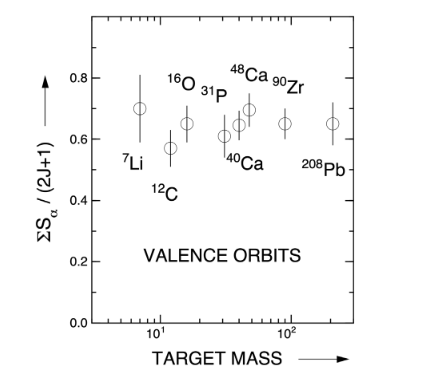
\includegraphics[width=0.9\linewidth]{figures/SF_aumann_review.png}
                \caption{T. Aumann \textit{et al.} Prog. Part. Nucl. Phys. 118 (2021)}
            \end{figure}
        \end{column}
    \end{columns}
\end{frame}

\begin{frame}{A long-standing puzzle}
    A trend with asymmetry $\Delta S \equiv S_{n} - S_{p}$ is found depending on the experimental \textbf{probe}!
    \begin{figure}
        \begin{tikzpicture}
            \node[anchor=south west,inner sep=0] (image) at (0,0) { 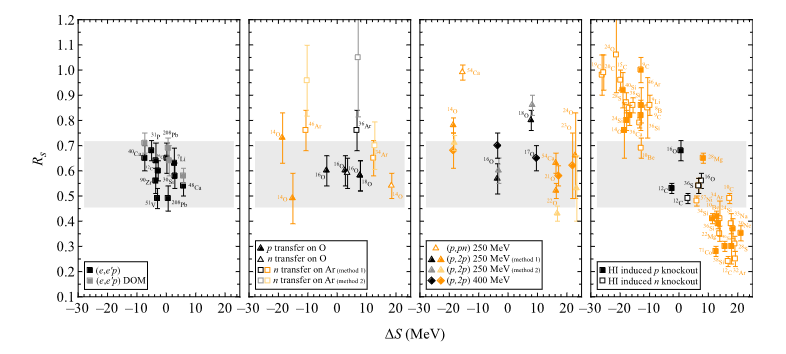
\includegraphics[width=0.9\linewidth]{figures/Rs_aumann_review.png}
            };
            \begin{scope}[x={(image.south east)},y={(image.north west)}]
                \node at (0.2, 0.85) {(e, e'p)};
                \node at (0.42, 0.85) {transfer};
                \node at (0.63, 0.85) {(p,2p)};
                \node[align=center] at (0.85, 0.85) {\textcolor{red}{Be-C} \\ \textcolor{red}{knock-out}};
                \draw[thick, red] (0.8, 0.7) -- (0.93, 0.32);
                % \draw[help lines,xstep=.05,ystep=.05] (0,0) grid (1,1);
                % \foreach \x in {0,1,...,9} { \node [anchor=north] at (\x/10,0) {0.\x}; }
                % \foreach \y in {0,1,...,9} { \node [anchor=east] at (0,\y/10) {0.\y}; }
            \end{scope}
        \end{tikzpicture}
        \caption{T. Aumann \textit{et al.} Prog. Part. Nucl. Phys. 118 (2021)}
    \end{figure}
    \mycolorbox{box2}{
        $\Rightarrow$ measure towards more exotic nuclei: \iso{10,12}{Be}!
    }
\end{frame}

\begin{frame}[t]{Importance of the overlaps}
    In a previous experiment by A. Matta and colleagues, for the $\iso{11}{Li}(d, \iso{3}{He})\iso{10}{Be}$ reaction they found that the \textbf{geometrical mismatch factor} (GMF) plays an essential role.
    \begin{columns}[T]
        \column{0.28\linewidth}
        {
            \begin{figure}
                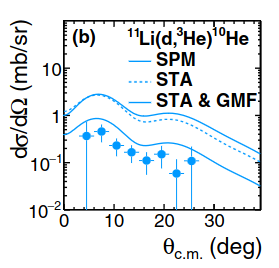
\includegraphics[width=0.9\linewidth]{figures/matta_11Li_d3He.png}
                \caption{A.Matta et al.}
            \end{figure}
        }
        \column{0.68\linewidth}
        {
            \begin{figure}
                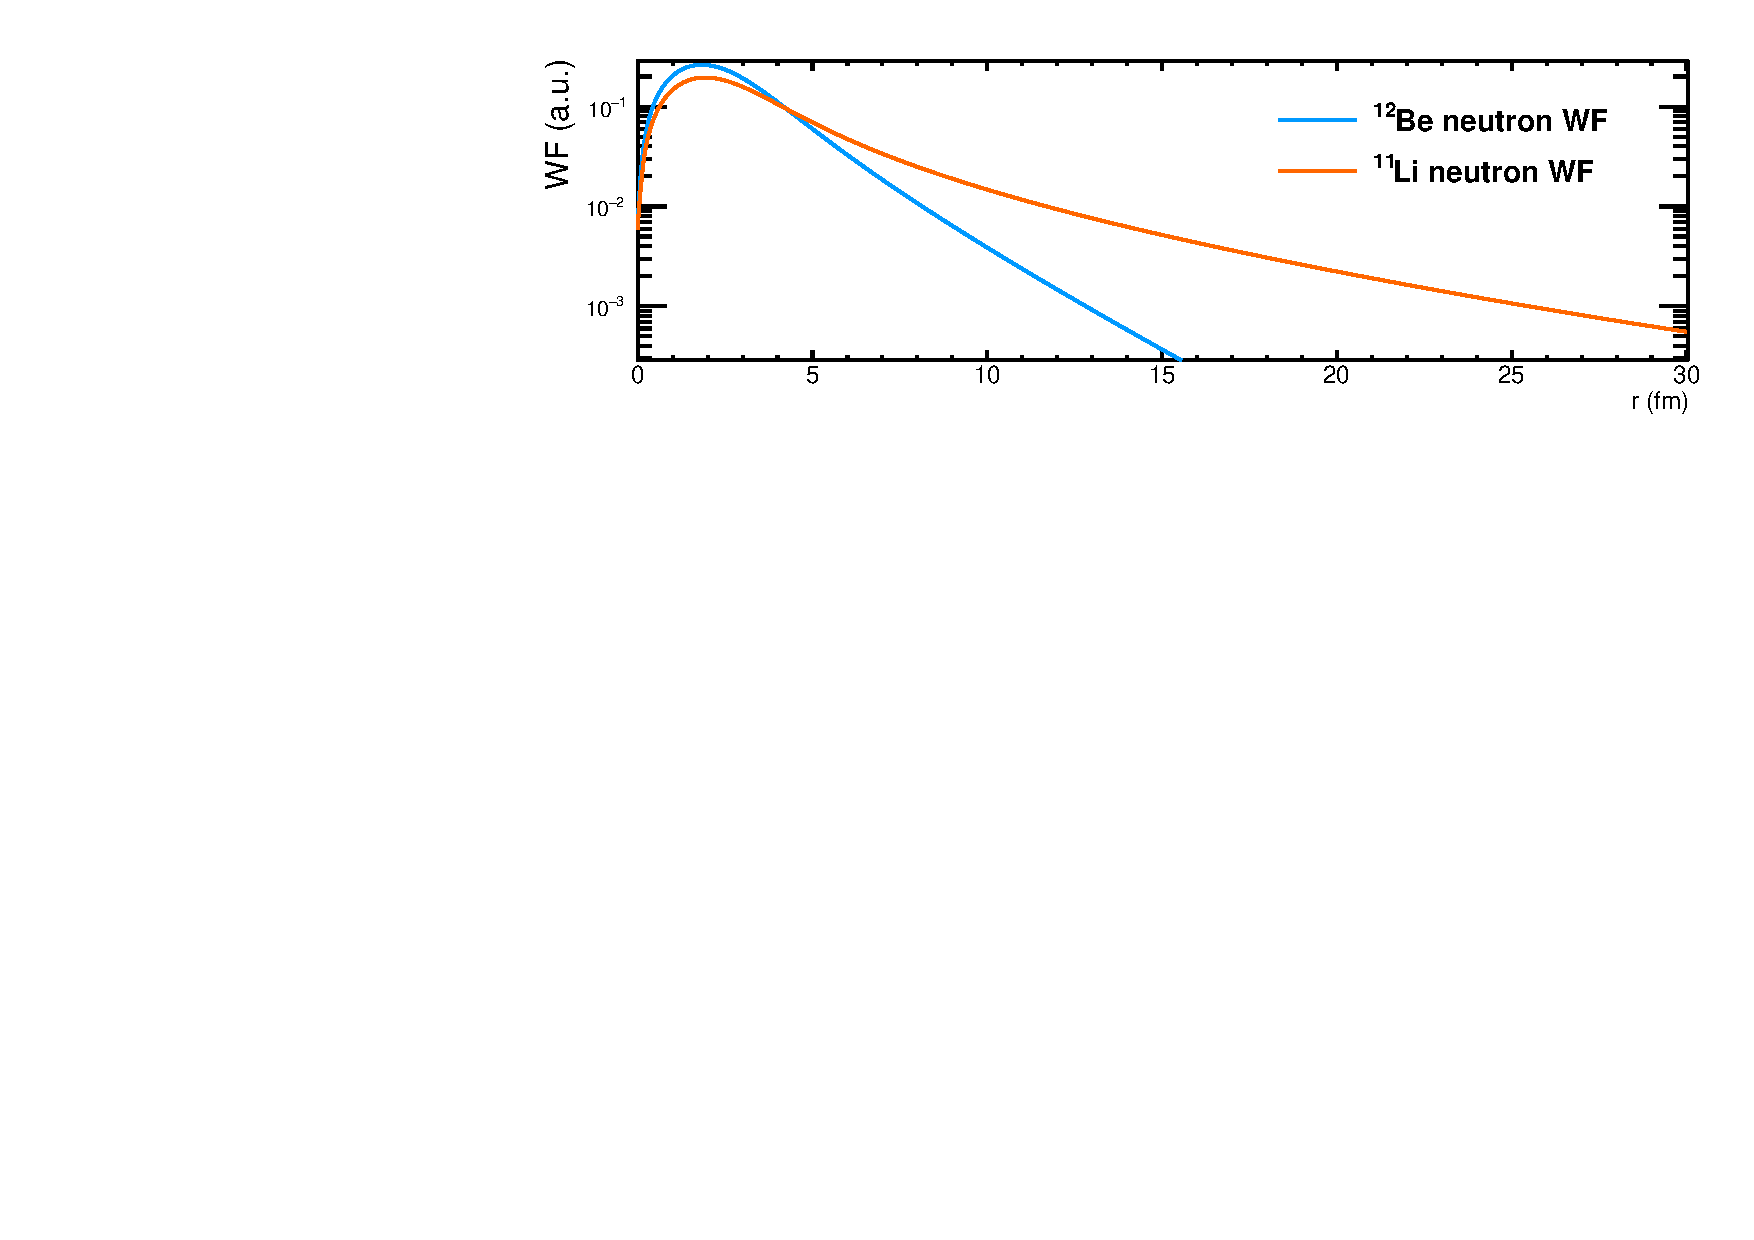
\includegraphics[width=1\linewidth]{figures/wf_12Be.pdf}
                \caption{A.Matta et al.}
            \end{figure}
        }
    \end{columns}

\end{frame}

\end{document}